\documentclass[17pt,a4paper,landscape]{extarticle}
\usepackage[margin=2.35cm,top=0.12cm,left=1.05cm]{geometry}
\usepackage{amsmath}
\usepackage{amssymb}
\usepackage{tasks}
\usepackage{tikz}
\usepackage{xcolor}
\usepackage[sfdefault,lf]{FiraSans}
\renewcommand{\familydefault}{\sfdefault}
\setlength{\parindent}{0pt}
\pagestyle{empty}
\settasks{label=\textbf{\arabic*.}, label-width=2.2em, item-indent=2.95em, column-sep=2.1cm, after-item-skip=4.7em}
\renewcommand{\arraystretch}{1.15}
\everymath{\displaystyle}

\begin{document}
\sffamily
\boldmath

\boldmath

\boldmath

{\LARGE \textbf{Angles on a straight line --- Foundation}}
\begin{tasks}(3)
\task {Find the missing angle.\\[0.4em]
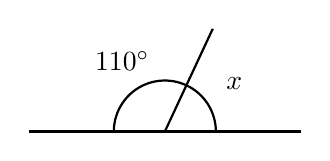
\begin{tikzpicture}[scale=0.72,baseline=(current bounding box.center)]
\draw[thick] (-2.4,0)--(0,0)--(2.4,0);
\draw[thick] (0,0)--({2*cos(65)},{2*sin(65)});
\draw[thick] (0.9,0) arc[start angle=0,end angle=65,radius=0.9];
\draw[thick] ({0.9*cos(65)},{0.9*sin(65)}) arc[start angle=65,end angle=180,radius=0.9];
\node at ({1.45*cos(32.5)},{1.45*sin(32.5)+0.06}) {$x$};
\node at ({1.4*cos(122.5)},{1.4*sin(122.5)+0.06}) {$110^\circ$};
\end{tikzpicture}}
\task {Find the missing angle.\\[0.4em]
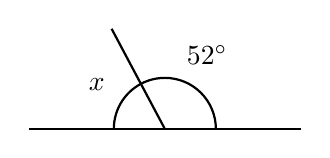
\begin{tikzpicture}[scale=0.72,baseline=(current bounding box.center)]
\draw[thick] (-2.4,0)--(0,0)--(2.4,0);
\draw[thick] (0,0)--({2*cos(118)},{2*sin(118)});
\draw[thick] (0.9,0) arc[start angle=0,end angle=118,radius=0.9];
\draw[thick] ({0.9*cos(118)},{0.9*sin(118)}) arc[start angle=118,end angle=180,radius=0.9];
\node at ({1.45*cos(59)},{1.45*sin(59)+0.06}) {$52^\circ$};
\node at ({1.4*cos(149)},{1.4*sin(149)+0.06}) {$x$};
\end{tikzpicture}}
\task {Find the missing angle.\\[0.4em]
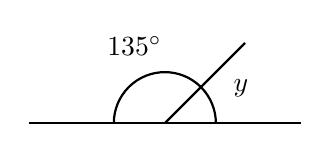
\begin{tikzpicture}[scale=0.72,baseline=(current bounding box.center)]
\draw[thick] (-2.4,0)--(0,0)--(2.4,0);
\draw[thick] (0,0)--({2*cos(45)},{2*sin(45)});
\draw[thick] (0.9,0) arc[start angle=0,end angle=45,radius=0.9];
\draw[thick] ({0.9*cos(45)},{0.9*sin(45)}) arc[start angle=45,end angle=180,radius=0.9];
\node at ({1.45*cos(22.5)},{1.45*sin(22.5)+0.06}) {$y$};
\node at ({1.4*cos(112.5)},{1.4*sin(112.5)+0.06}) {$135^\circ$};
\end{tikzpicture}}
\task {Find the missing angle.\\[0.4em]
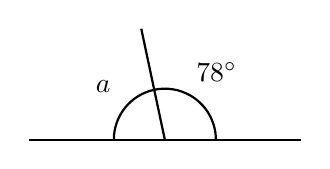
\begin{tikzpicture}[scale=0.72,baseline=(current bounding box.center)]
\draw[thick] (-2.4,0)--(0,0)--(2.4,0);
\draw[thick] (0,0)--({2*cos(102)},{2*sin(102)});
\draw[thick] (0.9,0) arc[start angle=0,end angle=102,radius=0.9];
\draw[thick] ({0.9*cos(102)},{0.9*sin(102)}) arc[start angle=102,end angle=180,radius=0.9];
\node at ({1.45*cos(51)},{1.45*sin(51)+0.06}) {$78^\circ$};
\node at ({1.4*cos(141)},{1.4*sin(141)+0.06}) {$a$};
\end{tikzpicture}}
\task {Find the missing angle.\\[0.4em]
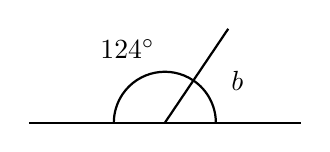
\begin{tikzpicture}[scale=0.72,baseline=(current bounding box.center)]
\draw[thick] (-2.4,0)--(0,0)--(2.4,0);
\draw[thick] (0,0)--({2*cos(56)},{2*sin(56)});
\draw[thick] (0.9,0) arc[start angle=0,end angle=56,radius=0.9];
\draw[thick] ({0.9*cos(56)},{0.9*sin(56)}) arc[start angle=56,end angle=180,radius=0.9];
\node at ({1.45*cos(28)},{1.45*sin(28)+0.06}) {$b$};
\node at ({1.4*cos(118)},{1.4*sin(118)+0.06}) {$124^\circ$};
\end{tikzpicture}}
\task {Find the missing angle.\\[0.4em]
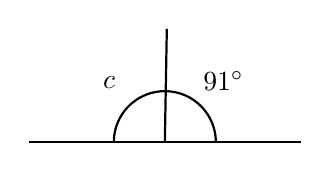
\begin{tikzpicture}[scale=0.72,baseline=(current bounding box.center)]
\draw[thick] (-2.4,0)--(0,0)--(2.4,0);
\draw[thick] (0,0)--({2*cos(89)},{2*sin(89)});
\draw[thick] (0.9,0) arc[start angle=0,end angle=89,radius=0.9];
\draw[thick] ({0.9*cos(89)},{0.9*sin(89)}) arc[start angle=89,end angle=180,radius=0.9];
\node at ({1.45*cos(44.5)},{1.45*sin(44.5)+0.06}) {$91^\circ$};
\node at ({1.4*cos(134.5)},{1.4*sin(134.5)+0.06}) {$c$};
\end{tikzpicture}}
\task {Find the missing angle.\\[0.4em]
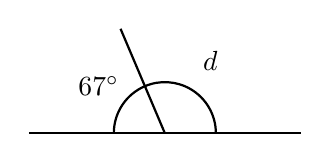
\begin{tikzpicture}[scale=0.72,baseline=(current bounding box.center)]
\draw[thick] (-2.4,0)--(0,0)--(2.4,0);
\draw[thick] (0,0)--({2*cos(113)},{2*sin(113)});
\draw[thick] (0.9,0) arc[start angle=0,end angle=113,radius=0.9];
\draw[thick] ({0.9*cos(113)},{0.9*sin(113)}) arc[start angle=113,end angle=180,radius=0.9];
\node at ({1.45*cos(56.5)},{1.45*sin(56.5)+0.06}) {$d$};
\node at ({1.4*cos(146.5)},{1.4*sin(146.5)+0.06}) {$67^\circ$};
\end{tikzpicture}}
\task {Find the missing angle.\\[0.4em]
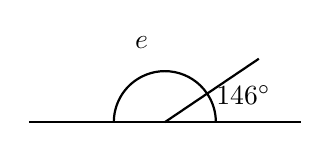
\begin{tikzpicture}[scale=0.72,baseline=(current bounding box.center)]
\draw[thick] (-2.4,0)--(0,0)--(2.4,0);
\draw[thick] (0,0)--({2*cos(34)},{2*sin(34)});
\draw[thick] (0.9,0) arc[start angle=0,end angle=34,radius=0.9];
\draw[thick] ({0.9*cos(34)},{0.9*sin(34)}) arc[start angle=34,end angle=180,radius=0.9];
\node at ({1.45*cos(17)},{1.45*sin(17)+0.06}) {$146^\circ$};
\node at ({1.4*cos(107)},{1.4*sin(107)+0.06}) {$e$};
\end{tikzpicture}}
\task {Find the missing angle.\\[0.4em]
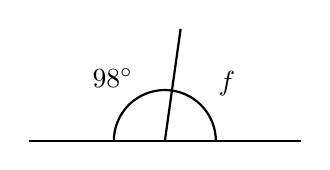
\begin{tikzpicture}[scale=0.72,baseline=(current bounding box.center)]
\draw[thick] (-2.4,0)--(0,0)--(2.4,0);
\draw[thick] (0,0)--({2*cos(82)},{2*sin(82)});
\draw[thick] (0.9,0) arc[start angle=0,end angle=82,radius=0.9];
\draw[thick] ({0.9*cos(82)},{0.9*sin(82)}) arc[start angle=82,end angle=180,radius=0.9];
\node at ({1.45*cos(41)},{1.45*sin(41)+0.06}) {$f$};
\node at ({1.4*cos(131)},{1.4*sin(131)+0.06}) {$98^\circ$};
\end{tikzpicture}}
\task {Are these angles on a straight line? Explain.\\[0.2em]\mbox{$95^\circ$} and \mbox{$85^\circ$}}
\task {Are these angles on a straight line? Explain.\\[0.2em]\mbox{$120^\circ$} and \mbox{$70^\circ$}}
\task {One angle is \mbox{$73^\circ$}. What is the angle next to it on the same straight line?}
\task {One angle is \mbox{$149^\circ$}. What is the angle next to it on the same straight line?}
\task {Complete the rule: angles on a straight line add to \mbox{$\underline{\hspace{1.5cm}}$}.}
\end{tasks}

\end{document}
